\section{Chapter Overview}
This chapter consists of the design decisions made to come up with a suitable architecture for implementation, based on the gathered requirements. High-level design, low-level design, design diagrams, UI wireframes have been used to convey how the design goals are expected to be achieved while discussing the reasoning for chosen design decisions.

\section{Design Goals}
% check non-functional requirements as well
% \setlength{\abovecaptionskip}{2pt plus 3pt minus 1pt} % Chosen fairly arbitrarily

\vspace{-4mm}       % remove line spacing after

% \begin{longtable}{|l|p{0.80\linewidth}|}
% \caption{Design Goals of the proposed system} \\
% \hline
% \textbf{Design Goal} & \textbf{Description} \\
% \hline
% \hline
% \end{longtable}

\begin{table}[h!]
\caption{Design Goals of the proposed system}
{\setstretch{1.5} 
\begin{tabular}{|l|p{0.81\linewidth}|}
\hline
\textbf{Design Goal} & \textbf{Description}\\
\hline
Performance & The recommendations matrix \& opinion-mining data can be pre-processed and stored in-memory to be used for recommendations. Since ensembled models are expected to be utilized, concurrency would be ideal to get the output from multiple models at the same time. This could cut down the processing time by 4-5 times (based on the number of models that are required to provide recommendations for the given input). \\ 
\hline
Correctness & The correctness \& quality of the output should be of the highest possible level, utilizing all the available data. By explaining why a user is getting the proposed recommendation will ensure that the user isn't mislead into wrong purchase decisions. \\ 
\hline
Usability & Since the purpose of the system is to automate and make it easy for the user to explore \gls{nft}s, the usability of the system must be easy for users of all levels of expertise. \\ 
\hline
Scalability & The system may have to support many concurrent user-requests in a production environment. The backend should be able to handle this. New data should be able to be added to the system with minimum effort. \\
\hline
Adaptability & Since the utilized Recommendation models may have to be altered based on the available data and user-requirements in the future, these models should be able to be easily swapped out for new models while ensuring that the system won't break in the process of upgrading, with minimum changes. \\
\hline
\end{tabular}
}
\end{table}

\section{High-Level Design}
% High-Level Design / System Architecture Design


\subsection{Tiered Architecture}

The system's architecture is depicted in the diagram below. The data, logic, and presentation layers are organized in a three-tier architecture.

The research contribution in this system lies in data preprocessing of the \textit{data tier}, recommendations models and in the recommendations diversifier of the \textit{logic tier}.


\begin{figure}[h!]
\centering
\frame{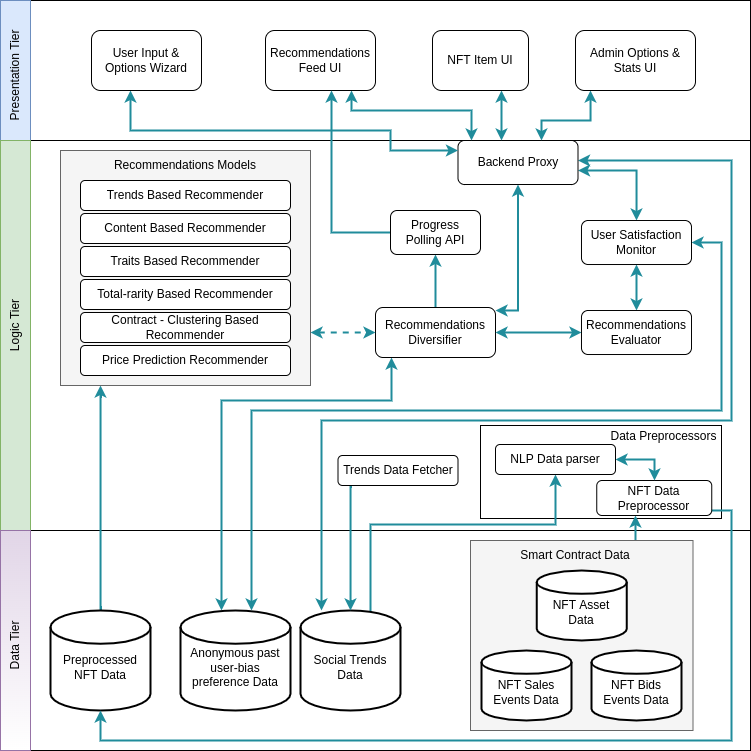
\includegraphics[width=\textwidth]{images/Design/tired-architecture-diagram.png}}
\caption{Three Tiered Architecture \textit{(self-composed)}}
\label{fig:three-tiered-architecuture}
\end{figure}

While the entire architecture is represented in a modular approach for ease of understanding, several backend services are expected to work together in the fashion of a distributed microservices architecture when it comes to implementating the proposed architecture.

The reason for following a microservices architecture is to allow the system to scale while ensuring that points of failure can be easily recognized and taken care of seperately. The distributed nature of the system is expected to be seen in the connection between the numerous Recommendations Models and the Recommendations Diversifier. These combined together through output-pipelines, will act as an Ensebled Recommendations System. Although the system will be capable of distributing the load at this point, the expectation with the prototype is to run this in a single machine.

The purpose of each module that is represented in the above architecture are described below.

\begin{enumerate}
\item Data Tier
%     \begin{enumerate}
%      \item Second level item
%      \item Second level item
%      \begin{enumerate}
%       \item Third level item
%       \item Third level item
%      \end{enumerate}
%   \end{enumerate}
\item Logic Tier
\item Presentation Tier (Client Tier)
\end{enumerate}



\subsection{Component Diagram}
% Is this necessary?


\section{Low-Level Design}
% Low-Level Design / System Design
\subsection{Choice of the Design Paradigm}
% SSADM seems to be the most suitable for this project- give reasons


\section{Design Diagrams}
% (component / class / sequence) - if OOP
% Any diagram that is relevant according to your choice of paradigm.

\subsection{Data Flow Diagram}

\subsection{Algorithm Design}

\subsection{UI Design}
% low fidelity wireframes

\subsection{System Process Flow Chart}

\section{Chapter Summary}
The design, architectural aspects and the flow of the project were documented in this chapter followed by the expected UI wireframes to be implemented for the end-user's interaction with the system.
